% Тут используется класс, установленный на сервере Papeeria. На случай, если
% текст понадобится редактировать где-то в другом месте, рядом лежит файл matmex-diploma-custom.cls
% который в момент своего создания был идентичен классу, установленному на сервере.
% Для того, чтобы им воспользоваться, замените matmex-diploma на matmex-diploma-custom
% Если вы работаете исключительно в Papeeria то мы настоятельно рекомендуем пользоваться
% классом matmex-diploma, поскольку он будет автоматически обновляться по мере внесения корректив
%

% По умолчанию используется шрифт 14 размера. Если нужен 12-й шрифт, уберите опцию [14pt]
%\documentclass[14pt]{matmex-diploma}
\documentclass[14pt]{matmex-diploma-custom}
\usepackage{multirow}
\begin{document}
% Год, город, название университета и факультета предопределены,
% но можно и поменять.
% Если англоязычная титульная страница не нужна, то ее можно просто удалить.
\filltitle{ru}{
    chair              = {Математическое обеспечение и администрирование информационных систем},
    title              = {Реализация поиска путей с регулярными и контекстно-свободными ограничениями в графовой базе данных RedisGraph},
    % Здесь указывается тип работы. Возможные значения:
    %   coursework - Учебная практика
    %   diploma - Диплом специалиста
        %   master - Диплом магистра
    %   bachelor - Диплом бакалавра
    type               = {practice},
    position           = {студента},
    group              = {343},
    author             = {Зиннатулин Тимур Раифович},
    supervisorPosition = {к.\,ф.-м.\,н., доцент кафедры информатики},
    supervisor         = {Григорьев\,С.\,В.},
    %reviewerPosition   = {ст. преп.},
    %reviewer           = {Привалов А.\,И.},
    %chairHeadPosition  = {д.\,ф.-м.\,н., профессор},
    %chairHead          = {Хунта К.\,Х.},
    university         = {Санкт-Петербургский Государственный Университет},
    city               = {Санкт-Петербург},
    year               = {2021}
}
\maketitle
\tableofcontents
% У введения нет номера главы
\section*{Введение}
Графовая модель представления данных~\cite{10.1145/298514.298576} является альтернативой реляционной модели. Её
особенность заключается в том, что данные представляются в виде графа. Его вершины
задают сущности модели. Они могут содержать в себе метки и свойства вида
"ключ-значение". Отношения, в свою очередь, задаются как ребра графа, которые
содержат в себе метку --- тип отношения. Графовые модели данных обладают большей
гибкостью во внесении изменений, чем реляционные, в связи с чем часто являются
приемлемым вариантом при проектировании баз данных. В частности, они успешно
используются в социальных сетях~\cite{social}, статическом анализе кода~\cite{URMA2015127} и др.

Одним из способов обработки информации в таких базах данных является поиск путей
между вершинами. В таком случае в запросе указываются ограничения на интересующие пользователя пути в графе.
Имеется множество подходов к заданию в графе путей с ограничениями. Один из таких
подходов исходит из теории формальных языков~\cite{forlangpath}. Пусть имеется помеченный 
граф, где метки являются символами некоторого алфавита. Тогда пути в графе соответствуют 
словам данного алфавита, так как являются последовательностью ребер с метками --- символами алфавита.
Далее, для введения ограничений на пути, задается грамматика, описывающая язык, 
содержащий только те слова, которые соответствуют нужным путям в графе.

Наибольший интерес среди таких грамматик представляют контекст-
но-свободные грамматики, так как они обладают большей выразительностью, чем регулярные грамматики. Они позволяют задавать более сложные отношения между вершинами в графе. К примеру, класс
запросов поиска вершин, лежащих на одном уровне иерархии~\cite{zhang2016contextfree}, задается
контекстно-свободными, но не регулярными ограничениями. Запросы такого типа находят
применение в биоинформатике~\cite{bioinf} и при анализе вершин в RDF-хранилищах~\cite{zhang2016contextfree}.

На данный момент в наиболее используемых графовых базах данных осуществляется
поддержка в лучшем случае регулярных ограничений, что сильно ограничивает
выразительность языка запросов. Когда возникает необходимость задавать к базе более сложные запросы, разработчикам приходится вручную писать алгоритмы для решения задачи контекстно-свободной достижимости для их частного случая.

Единственная полноценная поддержка контекстно-свободных запросов была реализована Арсением Тереховым~\cite{Arseniy-diploma} на основе графовой базы данных RedisGraph~\cite{RedisGraph}. В ней используется алгоритм Рустама Азимова~\cite{azimov-algo}, основанный на матричных операциях. На практике этот алгоритм является одним из самых быстрых алгоритмов выполнения контекстно-свободных запросов. Но для завершения интеграции алгоритма требуется написать тесты на корректность работы нововведенной функциональности, расширить валидацию запросов, поддерживаемых новым синтаксисом, а также обновить версию RedisGraph до более современной.
В данной работе будет завершено внедрение матричного алгоритма в RedisGraph и проведено исследование полученной реализации в реальных условиях.
 
\section{Постановка цели и задач}
Целью данной работы является полная интеграция матричного алгоритма в RedisGraph и исследование его производительности. Для достижения цели были поставлены следующие
задачи.
\begin{itemize}
    \item Улучшить имеющуюся поддержку базой данных RedisGraph запросов с контекстно-свободными ограничениями.
    \item Внедрить реализацию матричного алгоритма в основной репозиторий RedisGraph.
    \item Исследовать производительность полученной реализации. 
\end{itemize}

\section{Обзор}
Для описания работы матричного алгоритма введем понятие ослабленной нормальной формы Хомского.\\
\textbf{Определение 2.1.}
Пусть G = $\langle\Sigma$,N,P,S$\rangle$ --- контекстно-свободная грамматика, тогда G находится в ослабленной нормальной форме Хомского (ОНФХ), если содержит только правила вида:
\begin{itemize}
    \item $A \rightarrow BC$, где $A, B, C \in N$
    \item $A \rightarrow a$, где $A \in N, a \in \Sigma$
    \item $A \rightarrow \epsilon$, где $A \in N$
\end{itemize}

ОНФХ отличается от нормальной формы Хомского наличием правил вида $A \rightarrow \epsilon$, где А --- любой нетерминал, то есть А не
обязательно является стартовым, а также допущением использовать
стартовый нетерминал в правых частях правил.\\

\subsection{Алгоритм, основанный на матричном умножении}
Алгоритм Рустама Азимова~\cite{azimov-algo} решения задачи контекстно-свободной достижимости основан на обычном произведении матриц, благодаря чему он достигает хорошей производительности. На вход алгоритму поступает помеченный граф, который представлен в виде набора булевых матриц смежности для каждой метки, и контекстно-свободная грамматика, представленная в ОНФХ.
 
Основная идея алгоритма заключается в рассмотрении отдельно
правил, где в правой части находится один терминал, вида $A \rightarrow a$, и
правил, где в правой части находятся два нетерминала, вида $A \rightarrow BC$.
Для первого типа правил о наличии искомого пути говорит наличие дуги с меткой в виде терминала $a$. Для второго типа правил предлагается
умножать матрицы смежности, соответствующие двум нетерминалам
$B$ и $C$. Такая операция позволяет соединить дугой вершины, между которыми есть путь, состоящий из 2 дуг, первая из которых с меткой $B$,
а вторая — с $C$, тем самым гарантируя обнаружение путей, выводимых
из нетерминала $A$.

\subsection{GraphBLAS}
GraphBLAS~\cite{Graphblas} --- это матричный фреймворк, позволяющий работать с графами в терминах линейной алгебры. Он задает набор базовых операций для разреженных матриц над полукольцами.

Стандарт GraphBLAS отлично подходит для реализации алгоритма, основанного на матричном умножении. В частности, при его реализации была использована библиотека SuiteSparse\footnote{SuiteSparse: A Suite of Sparse Matrix Software: \url{https://people.engr.tamu.edu/davis/suitesparse.html} Accessed: 2021-11-11}, реализующая стандарт GraphBLAS. Эта библиотека является многопоточной и хорошо оптимизирована, что позволяет добиться высокой производительности.

\subsection{RedisGraph}
RedisGraph~\cite{RedisGraph} --- это высокопроизводительная графовая база данных, поддерживающая язык запросов Cypher. RedisGraph работает с графами в виде разреженных матриц смежности и транслирует запросы языка Cypher в матричные выражения.

Из-за представления графов в виде разреженных матриц смежности RedisGraph идеально подходит для реализации на его основе матричного алгоритма, в связи с чем была выбрана для полноценной реализации этого алгоритма на основе графовой базы данных. 

В рамках работы Арсения Терехова~\cite{Arseniy-diploma} была реализована поддержка матричного алгоритма. До полного внедрения требуется написать тесты на работоспособность новой функциональности и расширить валидатор запросов.


\section{Описание реализации}
В рамках учебной практики была улучшена текущая реализация матричного алгоритма на базе RedisGraph: были написаны тесты для проверки работоспособности алгоритма и был расширен валидатор запросов.
\subsection{Тесты}
В RedisGraph тестирование корректности запросов релазиовано на языке Python с использованием библиотеки RLTest\footnote{RLTest --- Redis Labs Test Framework: \url{https://github.com/RedisLabsModules/RLTest} Accessed: 2020-12-14}, разработанной компанией RedisLabs.

К тестовому графу делаются запросы на языке Cypher с реализованным синтаксисом из работы прошлого года~\cite{Timur-diploma}. Проверку проходят как обычные шаблоны путей, так и реализованные с их помощью контекстно-свободные запросы.

Также после тестирования с помощью библиотеки Valgrind\footnote{Valgrind --- system for debugging and profiling Linux programs: \url{https://valgrind.org/} Accessed: 2020-12-14} проводится проверка на утечки памяти. 

\subsection{Валидация запросов}
В RedisGraph основной частью обработки запроса является построение плана его выполнения. Её часть, которая относится к работе с контекстно-свободными ограничениями, приведена на рисунке~\ref{valid}. 
В ней зелёным цветом выделено то, что
было добавлено или расширено в работе~\cite{Arseniy-diploma}.
Сразу после получения запроса на языке Cypher строится абстрактное синтаксическое дерево~(АСТ). Перед тем, как строить что-либо по полученному дереву, необходимо провести его валидацию --- проверку на корректность введенного запроса. Желтым цветом выделен этап валидации, который был реализован для нового синтаксиса языка Cypher.

\begin{figure}[h]
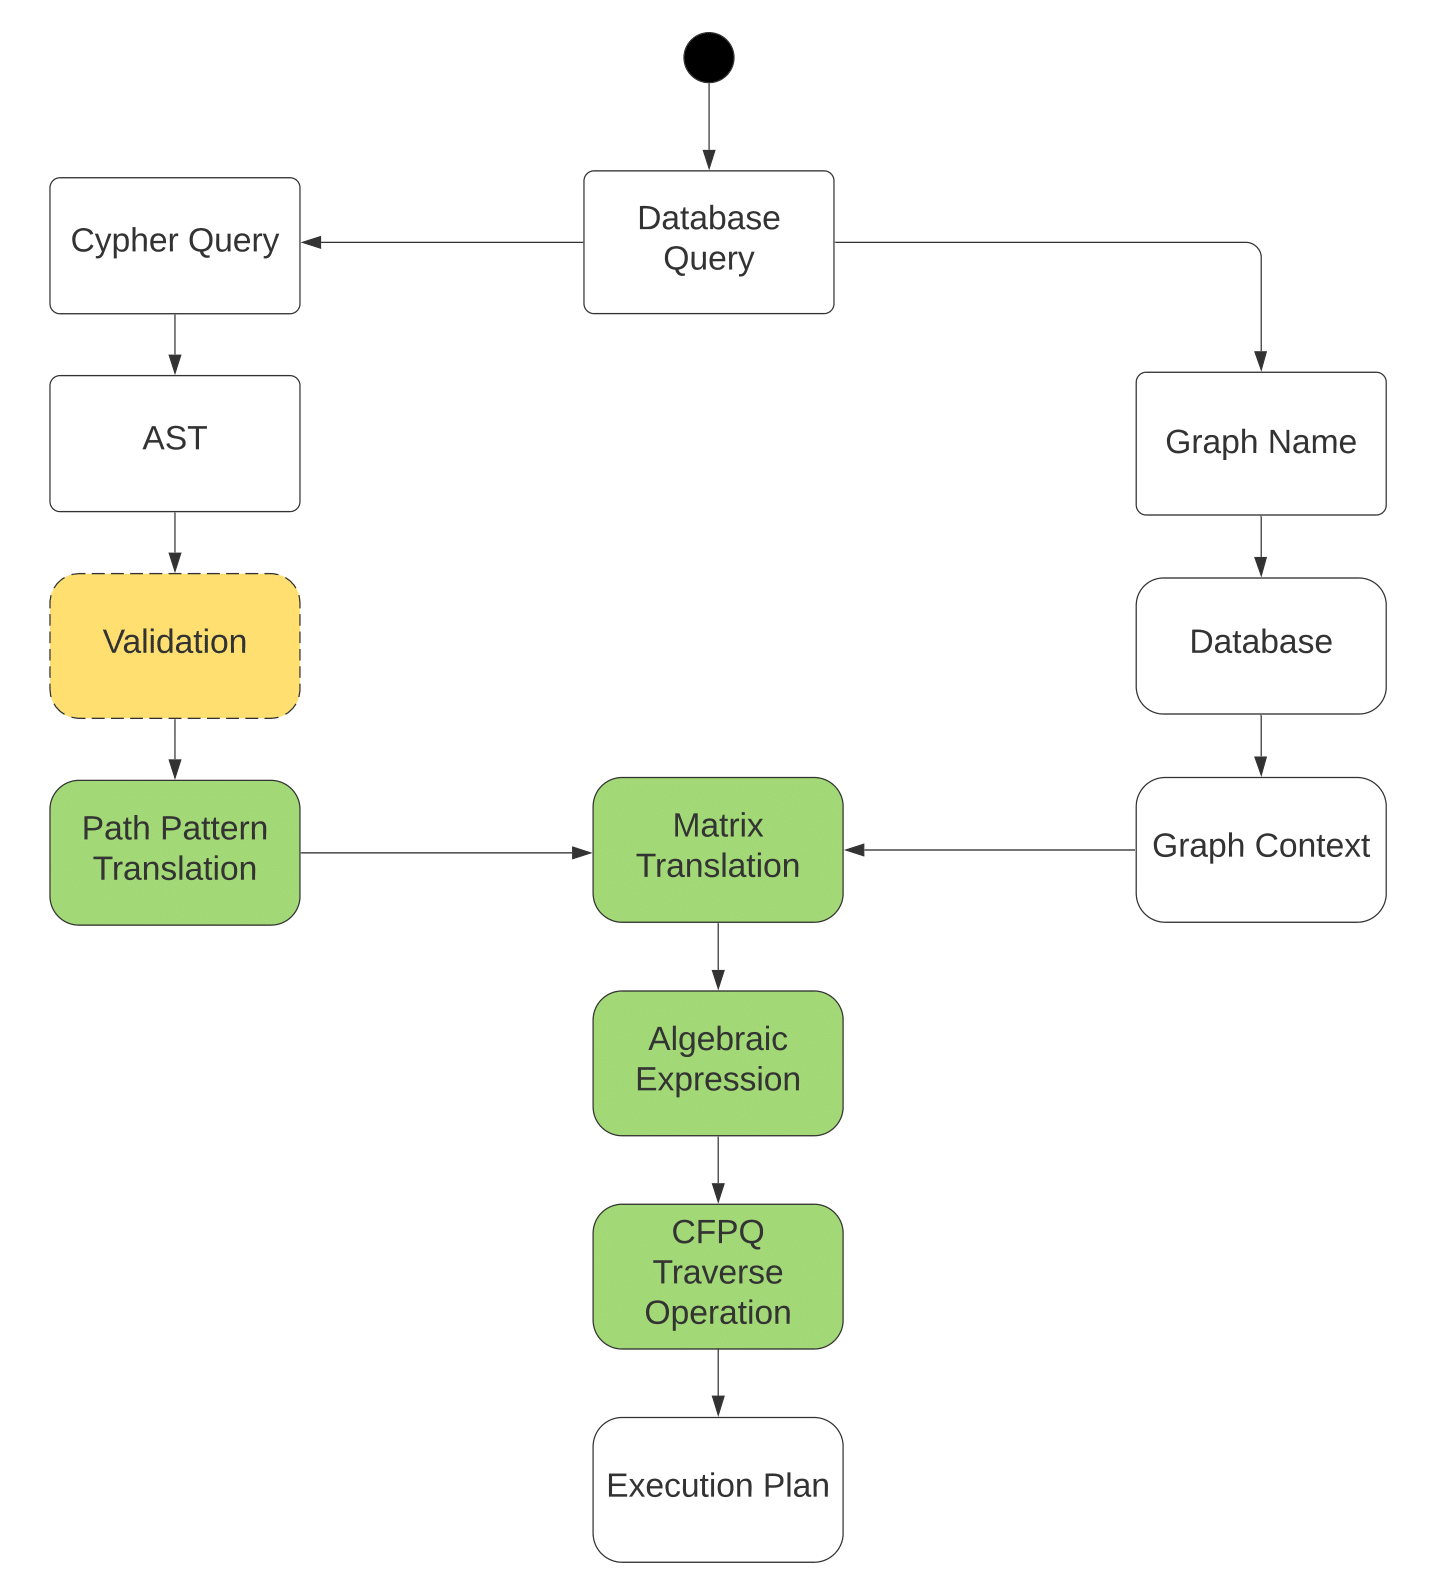
\includegraphics[width=12cm]{pictures/RedisGraph Activity Diagram-1.png}
\centering
\captionsetup{justification=centering}
\caption{Улучшение поддержки базой данных RedisGraph контекстно-свободных запросов}
\label{valid}
\end{figure}

Программа валидации запросов написана на языке C. В ней задействуется реализация библиотеки libcypher-parser, описанная в работе~\cite{Timur-diploma}. Эта библиотека предназначена для разбора языка Cypher в абстрактное синтаксическое дерево и его анализа\footnote{Используемая версия: \url{https://github.com/YaccConstructor/libcypher-parser/tree/path-patterns-support-for-redisgraph} Accessed: 2020-12-14}. 

Валидатор был расширен до состояния поддержки всех возможных вариантов поддерева АСТ, отвечающих за запросы с контекстно-свободными ограничениями.

\subsection{Интеграция с RedisGraph}
Была проведена работа по интеграции в текущую на тот момент версию RedisGraph. По итогу работы Арсением Тереховым был создан pull request\footnote{Pull request: \url{https://github.com/RedisGraph/RedisGraph/pull/1640} Accessed: 2021-10-10} в исходный репозиторий. 

\subsection{Доработка реализации}
Также было замечено, что в полученной реализации при вычислении транзитивного замыкания использовалось полукольцо LOR\_LAND, в то время как полукольцо ANY\_PAIR в контексте использования в реализации алгоритма выполняет те же функции, что и LOR\_LAND, но его операторы считают значения быстрее\footnote{SuiteSparse User Guide:\url{https://fossies.org/linux/SuiteSparse/GraphBLAS/Doc/GraphBLAS\_UserGuide.pdf} Accessed: 2021-11-11}.

Вследствие этого была создана еще одна версия реализации матричного алгоритма, где при вычислении транзитивного замыкания вместо полукольца LOR\_LAND было использовано полукольцо ANY\_PAIR, что потенциально должно было ускорить работу алгоритма.

\section{Эксперименты}
После завершения интеграции для двух полученных решений были произведены замеры производительности при обработке запросов с регулярными грамматиками. Затем на одной из реализаций было проведено исследование производительности на запросах с контекстно-свободными ограничениями.

Для проведения экспериментов с над полученной реализацией был использован ПК с операционной системой Ubuntu 18.04 и конфигурацией: Intel(R) Core(TM) i7-4790 CPU @ 3.60GHz CPU, DDR4 64 Gb RAM. Нижепредставленные графы и грамматики для построения шаблонов путей были взяты из набора данных CFPQ\_Data\footnote{CFPQ\_Data: Data for Context-Free Path Querying Evaluation: \url{https://jetbrains-research.github.io/CFPQ\_Data/index.html} Accessed: 2021-10-11}, собранного исследователями лаборатории языковых инструментов JetBrains
Research.  

\subsection{Сравнение реализаций на регулярных запросах}
Для запросов с регулярными ограничениями был выбран граф geospecies. Этот граф использовался для исследования алгоритма, основанного на тензорном произведении~\cite{tensoralgo} и оказался одним из наиболее показательных графов на регулярных запросах. Метаданные графа geospecies представлены в таблице~\ref{tab:geospecies}.

По этому графу была сгенерирована статистика количества вхождения меток ребер, и самые частовстречающиеся из них были выбраны как символы алфавита. По этому алфавиту были составлены регулярные выражения, которые использовались для задания запросов. Эти выражения представлены в таблице~\ref{tab:regex}.

\begin{table}[h!]
    \centering
    \begin{tabular}{|c||c|c|c|c|c|}
        \hline
         Graph name & \#vertices & \#edges & \#A & \#B & \#C \\
        \hline \hline
         geospecies & 450 609 & 2 201 532 & 127 098 & 127 055 & 109 608\\
         \hline
    \end{tabular}
    \caption{Метаданные используемого графа}
    \label{tab:geospecies}
\end{table}

На рис.~\ref{rpq} представлен вид запроса на языке Cypher с расширенным синтаксисом, задающий ограничение на пути в виде регулярного выражения $Q_2$.
\begin{table}[h!]
    \centering
    \begin{tabular}{|c||c|}
        \hline
        Name & Query \\
        \hline
        Q_1 & A* \\
        Q_2 & A $\cdot$ B* \\
        Q_3 & A $\cdot$ B* $\cdot$ C* \\
        Q_4 & (A | B)* \\
        Q_5 & A $\cdot$ B* $\cdot$ C \\
        Q_6 & A* $\cdot$ B* \\
        Q_7 & A $\cdot$ B $\cdot$ C* \\
        \hline
    \end{tabular}
    \caption{Регулярные выражения для задания запрсов}
    \label{tab:regex}
\end{table}

\begin{figure}[h!]
    \begin{verbatim}
        PATH PATTERN S = ()-/ :A :B* /->()
        MATCH ()-/ ~S /->()
        RETURN COUNT(*)
    \end{verbatim}
    \caption{Вид запроса на примере Q_2}
    \label{rpq}
\end{figure}

\begin{table}[h!]
    \centering
    \begin{tabular}{ |c||c|c|c|c|c| }
        \hline
         \multirow{2}{*}{Query} & \multirow{2}{*}{Result} & \multicolumn{2}{|c|}{Binary\_Op} & \multicolumn{2}{|c|}{Any\_Pair}\\
         \cline{3---6} & & time(s) & SD(s) & time(s) & SD(s) \\
         \hline
         Q_1 & 577 707 & 20,9 & 0,2 & 20,9 & 0,1\\
         Q_2 & 6 588 862 & 8,7 & 0,1 & 8,7 & 0,1\\
         Q_3 & 6 779 512 & 24,0 & 0,2 & 24,0 & 0,2\\
         Q_4 & 7 280 991 & 55,4 & 0,2 & 55,3 & 0,1\\
         Q_5 & 15 252 & 8,6 & 0,1 & 8,6 & 0,1\\
         Q_6 & 7 163 984 & 56,0 & 0,0 & 56,0 & 0,1 \\
         Q_7 & 6 652 414 & 11,7 & 0,0 & 11,6 & 0,0 \\
         \hline
    \end{tabular}
    \caption{Сравнение разных версий RedisGraph на регулярных запросах}
    \label{tab:redisgraph_rpq}
\end{table}

%Таблица с временем выполнения запросов
 Для каждой версии RedisGraph создавался отдельный docker-образ, на который посылались запросы. Каждый запрос запускался 5 раз, и время его работы усреднялось. Результирующее время было взято с точностью до десятых.
 
В таблице~\ref{tab:redisgraph_rpq} представлены результаты замеров регулярных запросов на двух разных версиях реализации матричного алгоритма в RedisGraph. В колонках "Binary\_Op" представлены время выполнения запросов $Q_{1..7}$ старой версией алгоритма и их стандартное отклонение в секундах, а в колонках "Any\_Pair" --- время работы версии алгоритма с использованием полукольца ANY\_PAIR и стандартное отклонение, также в секундах.

Эксперименты показали, что использование полукольца ANY\_PAIR никак ощутимо не повлияло на время исполнения запросов с регулярными ограничениями. В дальнейшем для замеров будет использована версия алгоритма с полукольцом ANY\_PAIR.

\subsection{Эксперименты с контекстно-свободными запросами}
Далее были проведено исследование работоспособности и производительности полностью интегрированного матричного алгоритма на базе RedisGraph при обработке контекстно-свободных запросов.

\subsubsection{MemoryAliases}
Для проведения замеров запросов с контекстно-свободными ограничениями были выбраны графы класса MemoryAliases --- графы, использующиеся для анализа указателей языка Си. Метаданные графов MemoryAliases представлены в таблице~\ref{tab:memoryal_meta}.

\begin{table}[h!]
    \centering
    \begin{tabular}{|c||c|c|c|c|}
         \hline
         Graph & \#vertices & \#edges & \#A & \#D \\
         \hline \hline
         wc & 332 & 269 & 113 & 156\\
         bzip2 & 632 & 556 & 259 & 297\\
         pr & 815 & 692 & 333 & 359\\
         ls & 1687 & 1453 & 703 & 750\\
         gzip & 2687 & 2293 & 1075 & 1218\\
         \hline
    \end{tabular}
    \caption{Метаданные графов MemoryAliases}
    \label{tab:memoryal_meta}
\end{table}

Запрос, используемый для замеров, представлен на рис.~\ref{memoryal_q}. Для каждого графа данный запрос запускался 5 раз, было взято среднее время работы с точностью до десятых.

\begin{figure}[h!]
    \begin{verbatim}
        PATH PATTERN V1 = ()-/ [ ~V2 <:A ~V1 ] | () /->()
        PATH PATTERN V2 = ()-/ ~S | () /->()
        PATH PATTERN V3 = ()-/ [ :A ~V2 ~V3 ] | () /->()
        PATH PATTERN S = ()-/ <:D ~V1 ~V2 ~V3 :D /->()
        MATCH ()-/ ~S /->()
        RETURN COUNT(*)
    \end{verbatim}
    \caption{Структура запроса для MemoryAliases}
    \label{memoryal_q}
\end{figure}

\begin{table}[h!]
    \centering
    \begin{tabular}{|c||c|c|c|}
        \hline
        Graph & Result & Time(ms) & SD(ms) \\
        \hline \hline
        wc & 156 & 33,1 & 1,2 \\
        bzip2 & 315 & 67,6 & 13,5 \\
        pr & 385 & 124,2 & 5,1 \\
        ls & 854 & 98,9 & 1,5 \\
        gzip & 1458 & 162,0 & 1,8 \\
        \hline
    \end{tabular}
    \caption{Результаты запросов к графам MemoryAliases}
    \label{tab:memoryal_res}
\end{table}

В таблице~\ref{tab:memoryal_res} представлены результаты экспериментов над графами MemoryAliases. Результаты экспериментов соотносятся с результатами, полученными в предыдущих исследованиях~\cite{memoryaliases}.
\subsubsection{RDF}
Также для исследования были взяты графы из набора RDF --- реальные биологические данные. Их метаданные представлены в таблице~\ref{tab:rdf_meta}. Для них были составлены классические запросы same-generation, используемые в других работах по исследованию запросов с контекстно-свободными ограничениями. Данные запросы представлены в синтаксисе Cypher на рис.~\ref{rdf_q}.
\begin{table}[h!]
    \centering
    \scalebox{0.8}{
    \begin{tabular}{|c||c|c|c|c|c|}
         \hline
         Graph & \#vertices & \#edges & \#SCO & \#T & \#BT \\
         \hline \hline
         pathways & 6238 & 12 363 & 3117 & 3118 & --- \\
         gohierarchy & 45 007 & 490 109 & 490 109 & --- & --- \\
         enzyme & 48 815 & 86 543 & 8163 & 14 989 & --- \\
         eclass514\_en & 239 111 & 360 248 & 90 962 & 72 517 & --- \\
         go & 582 929 & 1 758 432 & 94 514 & 226 481 & --- \\
         geospecies & 450 609 & 2 201 532 & --- & 89 062 & 20 867 \\
         \hline
    \end{tabular}}
    \caption{Метаданные графов с RDF-данными}
    \label{tab:rdf_meta}
\end{table}\\

\begin{figure}[h!]
    \begin{verbatim}
        #Query_1
        PATH PATTERN S1 = ()-/ [ <:SCO [ ~S1 | () ] :SCO ] |
                              [ <:T [ ~S1 | () ]  :T ] /->()
        MATCH ()-/ ~S1 /->()
        RETURN COUNT(*)
        
        #Query_2
        PATH PATTERN S2 = ()-/ <:SCO [ ~S2 | () ] :SCO /->()
        MATCH ()-/ ~S2 /->()
        RETURN COUNT(*)
        
        #Query_geo
        PATH PATTERN S3 = ()-/ :BT [ ~S3 | () ]  <:BT /->()
        MATCH ()-/ ~S3 /->()
        RETURN COUNT(*)
    \end{verbatim}
    \caption{Запросы same-generation}
    \label{rdf_q}
\end{figure}

Замеры по каждому графу и каждому запросу проводились таким же образом, как в испытаниях на графах MemoryAliases.\\
\begin{table}[h!]
    \centering
    \scalebox{0.75}{
    \begin{tabular}{|c||c|c|c||c|c|c||c|c|c|}
        \hline
         \multirow{2}{*}{Graph} & \multicolumn{3}{|c||}{Query\_1} & \multicolumn{3}{|c||}{Query\_2} & \multicolumn{3}{|c|}{Query\_geo}\\
         \cline{2---10}
         & result & time(s) & SD(s) & result & time(s) & SD(s) & result & time(s) & SD(s)\\
         \hline \hline
         pathways & 884 & 0,1 & 0,0 & 887 & 0,1 & 0,0 & --- & --- & ---\\
         gohierarchy & 588 976 & 0,8 & 0,0 & 588 976 & 0,7 & 0,0 & --- & --- & ---\\
         enzyme & 396 & 0,3 & 0,0 & 394 & 0,2 & 0,0 & --- & ---& ---\\
         eclass514\_en & 90 994 & 6,7 & 0,0 & 90 988 & 4,1 & 0,0 & --- & ---& ---\\
         go & 640 316 & 149,3 & 0,6 & 640 305 & 96,9 & 0,1 & --- & --- & ---\\
         geospecies & 85 & 6,5 & 0,1 & --- & --- & --- & 226 669 749 & 58,1 & 0,8\\
         \hline
         
    \end{tabular}}
    \caption{Результаты экспериментов с контекстно-свободными запросами к RDF-данным}
    \label{tab:rdf_res}
\end{table}

Результаты экспериментов соотносятся с результатами, полученными в предыдущих исследованиях, проведенных на этих наборах данных~\cite{Arseniy-diploma}. Время исполнения запросов на RedisGraph с полностью интегрированным алгоритмом больше, чем в других исследованиях~\cite{azimov-algo} того же алгоритма, но это ожидаемый результат в силу издержек, возникающих при выполнении запроса внутри графовой базы данных.

В дальнейшем требуется сравнить скорость работы полученной реализации с другими графовыми базами данных, поддерживающими запросы с регулярными ограничениями.

% У заключения нет номера главы
\section*{Заключение}
В рамках учебной практики были выполнены следующие задачи:
\begin{itemize}
    \item Улучшена имеющаяся поддержка базой данных RedisGraph запросов с контекстно-свободными ограничениями.
    \item Завершено внедрение матричного алгоритма в RedisGraph.
    \item Проведено экспериментальное исследование производительности полученной реализации.
    \item Результаты работы изложены в статье "Multiple-Source Context-Free Path Querying in Terms of
Linear Algebra", опубликованной на конференции EDBT 2021
\end{itemize}

В дальнейшем планируется продолжить проведение экспериментального исследования производительности алгоритма на регулярных запросах и контекстно-свободных запросах и сравнить результаты с существующими аналогами. Также в будущем планируется разработать подробную пользовательскую документацию запросов в расширенном синтаксисе Cypher.

Текущее состояние репозитория можно увидеть на GitHub\footnote{Рабочая ветвь: \url{https://github.com/YaccConstructor/RedisGraph/tree/any_pair_traversal} Accessed: 2021-11-04.}.
\setmonofont[Mapping=tex-text]{CMU Typewriter Text}
\bibliographystyle{ugost2008ls}
\bibliography{diploma.bib}
\end{document}
